
\section{Overview}\label{sect:Overview}

This tutorial is intended to provide a introduction to the basics of Markov chain Monte Caro (MCMC) using the  Metropolis-Hastings algorithm. This will provide a brief introduction to MCMC moves as well as prior distributions. We begin with a simple example of estimating the probability distribution of an archer's ability to shoot at a target, and the distance those arrows land from the center. We will simulate data using this example and attempt to estimate the posterior distribution using a variety of MCMC moves. 

\bigskip
\subsection{Learning Outcomes}
\begin{itemize}
\item Understand and implement the Metropolis-Hastings MCMC algorithm
\item Begin to develop an intuition regarding the use of different priors 
\item Understand the difference and utility of various MCMC moves 
\end{itemize}

\subsection{Required Software}\label{subsect:Overview-Requirements}

This tutorial requires that you download and install the latest release of \RevBayes \citep{Hoehna2017a}, which is available for Mac OS X, Windows, and Linux operating systems. 
Directions for downloading and installing the software are available on the program webpage:
%\begin{center}
\href{http://revbayes.com/}{http://revbayes.com}.
%\end{center} 

The exercise provided also requires additional programs for editing text files and visualizing output. 
The following are very useful tools for working with \RevBayes:
\begin{itemize}[noitemsep,topsep=0pt]
\item A good text editor -- if you do not already have one that you like, we recommend one that has features for syntax coloring, easy navigation between different files, line numbers, etc.
Good options include \href{http://www.sublimetext.com/}{\tt Sublime Text} or \href{https://atom.io/}{Atom}, which are available for Mac OSX, Windows, and Linux.
\item \href{http://tree.bio.ed.ac.uk/software/tracer/}{\tt Tracer} -- for visualizing and assessing numerical parameter samples from \RevBayes
\end{itemize}

\bigskip
\section{Introduction}\label{sect:Introduction}




\newpage
\section{Modeling an archer's shots on a target}\label{sect:Exercise}

Suppose you are interested in estimating the distribution of an archer's shots on a target. For simplicity we will assume that these $n$ shots are all taken from 10 meters away from the target by the same experienced archer. One way that we could do this is to measure how far each arrow lands from the bullseye. Let's assume that these distances follow a truncated normal distribution with some mean, $\mu$, and some standard deviation, $\sigma$, and a minimum of $0$ meters, and a maximum of $300$ meters. For Bayesian inference it is often more convinient to reparameterize the standard deviation as $\tau = \frac{1}{\sigma^2}$. The following represents the data model for $n$ arrows shot where $a$ is a data point and $\Phi$ is the cumulative distribution function of the standard normal distribution:
\[ p(a_i | \mu, \tau, 0, 300) = \prod_{i=1}^{n} \frac{\frac{\sqrt{\tau}}{\sqrt{2\pi}} exp\left(-\frac{1}{2}\tau(a_i - \mu)^2\right)}{(\Phi(300) - \Phi(0))} \]

Now suppose we don't know what the mean is, but we do know the standard deviation for simplicity. Now we need to place a prior on the mean that describes our uncertainty about the mean. For now let's use another truncated normal distribution and so our prior becomes:
\[ p(\mu | \mu_0, \sigma_0, 0, 300) = \frac{\frac{\sqrt{\tau_0}}{\sqrt{2\pi}}exp\left(-\frac{1}{2}\tau_0(\mu - \mu_0)^2\right)}{(\Phi(300) - \Phi(0))} \]
where $\mu_0$ and $\sigma_0$ are set by the scientist. The values of these should reflect one's belief about the parameter that the prior distribution distribution. For example, if we were very confident then we would set both $\mu_0$ and $\sigma_0$ to a small numbers. Intuitively, it may be useful to think of the $\mu_0$ as your guess about the parameter and $\sigma_0$ as your confidence in that guess. Using Bayes' Rule we can then derive the posterior: 

\[ p(\mu | y, \sigma) = \frac{\frac{\sqrt{\tau_n}}{\sqrt{2\pi}}exp\left(-\frac{1}{2}\tau_n(\mu - \mu_n)^2\right)}{ (\Phi(300) - \Phi(0))} \]

with
\[ \mu_n = \tau_n^{-1} (n\tau \bar{a} + \sigma_0 \mu_0) \]
   \[\tau_n = \tau_0 + n\tau \]
   \[\bar{a} = \frac{1}{n}\sum_{i=1}^{n} x_i\]

As you can see the posterior distribution has the same distribution family as the prior. When this happens the prior is called the conjugate prior distribution. In addition, the normal prior for this model has the attractive property that its posterior precision is the sum of the prior mean and the data mean, and the posterior mean is the precision weighted average of the prior mean and the data mean.


\medskip
\subsection{Tutorial Format}\label{subsect:Exercise-Format}

This tutorial follows a specific format for issuing instructions and information.

{\begin{framed}
The boxed instructions guide you to complete tasks that are not part of the \RevBayes syntax, but rather direct you to create directories or files or similar.
\end{framed}}

Information describing the commands and instructions will be written in paragraph-form before or after they are issued.

All command-line text, including all \Rev syntax, are given in \cl{monotype font}. 
Furthermore, blocks of \Rev code that are needed to build the model, specify the analysis, or execute the run are given in separate shaded boxes.
For example, we will instruct you to create a constant node called \cl{rho} that is equal to \cl{1.0} using the \cl{<-} operator like this:
{\tt \begin{snugshade*}
\begin{lstlisting}
rho <- 1.0 # constant node
alpha ~ dnExponential(rho) # stochastic node
lambda := 1 / alpha # deterministic node
\end{lstlisting}
\end{snugshade*}}

It is important to be aware that some PDF viewers may render some characters given as \colorbox{shadecolor}{\tt{Rev commands}} differently. 
Thus, if you copy and paste text from this PDF, you may introduce some incorrect characters. 
Because of this, we recommend that you type the instructions in this tutorial or copy them from the scripts provided. 


\medskip
\subsection{Data and Files}\label{subsect:Exercise-DataFiles}

{\begin{framed}
On your own computer or your remote machine, create a directory called {\textcolor{red}{\cl{RB\_MyFirstMCMC\_Tutorial}}} (or any name you like).

\end{framed}}

In this tutorial we will be simulating our own data using \RevBayes. Explain how to simulate data in Rev. We will be simulating data. Let's assume from the above archery example that our archer's true ability has their arrows landing with a mean of 0 and a variance of 1. Let's say they shoot six arrows. We do this in \RevBayes like this:

 {\tt \begin{snugshade*}
\begin{lstlisting}
minimum = 0
maximum = 300
num_arrows = 6
true_mu = 0.0
true_var = 1

arrows = rnormal(n = num_arrows, mean = true_mu, sd = true_sd, min = minimum, max = maximum)

\end{lstlisting}
\end{snugshade*}}



\bigskip
\subsection{Getting Started with MCMC\label{subsect:Exercise-GetStart}}

As you saw above, we were able to get a nice analytical posterior distribution for our normal model with known variance and a normal prior on the mean even in the case of a truncated normal. However, in the majority of interesting scientific cases we are unable to do this. This is where MCMC comes in. MCMC algorithms are a set of tools that provide us with a means to estimate the posterior even in very complex scenarios. There are many flavors of MCMC algorithms; however, this tutorial will only cover the Metropolis-Hastings algorithm. The basic idea of this algorithm is to propose new values for our parameter, $\theta$, in some way (here they are termed moves) Then based on our data model and prior we calculate what is called the Hastings ratio:

\[ R = \frac{p( y | \theta^\prime  ) p(\theta^\prime) }{p( y | \theta ) p(\theta)}  \times \frac{ q( \theta | \theta^\prime )} { q( \theta^\prime | \theta) } \]

where $\theta^\prime$ represents the new proposed value of the parameter and $\theta$ represents the previous iteration's value. $q(\theta^\prime | \theta)$ is called the proposal distribution. However, oftentimes it is convenient to choose our proposals such that $ q(\theta^\prime | \theta) = q(\theta | \theta^\prime)$ thus eliminating that term from the calculation of $R$, moves that have this property are called symmetric moves. The Hastings ratio is then used to determine whether the proposed value, $\theta^\prime$ is an improvement over the previous iterations value. 

The Metropolis-Hastings algorithm is stated as follows:
\begin{enumerate}
\item Set an initial value for $\theta$
\item Draw a new value, $\theta^\prime$ from $q(\theta^\prime | \theta)$
\item Calculate the Hastings ratio
\item Draw $u$ from $Unif(0,1)$ 
\item If $u < R$ then we set $\theta = \theta^\prime$ 
\item Record the value of $\theta$ and go to 2. Repeating $N$ times
\end{enumerate}



\subsubsection{Metropolis-Hastings algorithm by hand}

Go through outline of algorithm steps. explain proposal distributions. Then go into a step-by-step on how to write a MH-algorithm in Rev. First write the functions for the likelihood and the prior. 

Likelihood function:

{\tt \begin{snugshade*}
\begin{lstlisting}
function Natural logLikelihood(mu_prime, sd_zero, mini, maxi){
	likelihood_mean = 0.0
	for(i in 1:num_arrows){
		likelihood_mean += dnormal(arrows[i], mu_prime, sd_zero, min = mini, max = maxi, log=true)
	}
	return likelihood_mean
}
\end{lstlisting}
\end{snugshade*}}

Prior function: 

{\tt \begin{snugshade*}
 \begin{lstlisting}
function Natural logPriorMean(mu_prime, mu_zero, sd_zero, mini, maxi){
	prior_mean = dnormal(mu_prime, mu_zero, sd_zero, min = mini, max = maxi, log=true)
	return prior_mean
}
\end{lstlisting}
\end{snugshade*}}



Draw an initial value for our mean from the prior distribution:

{\tt \begin{snugshade*}
 \begin{lstlisting}
prior_mu = 0.5
stdev = 1
mu <- rnorm(1, mean = prior_mu, stdev, min = minimum, max= maximum)
\end{lstlisting}
\end{snugshade*}}

Set number of iterations of our MCMC and setup writing our output:

{\tt \begin{snugshade*}
 \begin{lstlisting}
reps = 10000
write("iteration","p","\n",file="output/archery_MH.log")
write(0,v,"\n",file="output/archery_MH.log",append=TRUE)
\end{lstlisting}
\end{snugshade*}}


Now before we write out MCMC algorithm. We need to decide what type of proposal we are going to use on our parameter, $\mu$. For new we will simply randomly propose new values for $\mu$ by taking our previous value of $\mu$ and adding a uniformly distributed variable to that value. The uniform distribution we use will be drawn from the range $\{ -\delta, \delta \}$ where $\delta$ is set to some value. This parameter, $\delta$, is known as a tuning parameter and can be optimized to allow for the most efficient sampling of our target distribution. Finally, we can write our Metropolis Hastings Algorithm:

{\tt \begin{snugshade*}
 \begin{lstlisting}
# first we need to set delta
delta = 0.1 

# the actual algorithm
for(rep in 1:reps){

	mu_prime = mu + runif(n=1, -delta, delta)[1] 

	R = (logLikelihood(mu_prime, stdev, minimum, maximum) - logLikelihood(mu, stdev, minimum, maximum)) +
		 ( logPriorMean(mu_prime, prior_mu, stdev, min = minimum, max = maximum) - logPriorMean(mu, prior_mu, stdev, min = minimum, max = maximum)) 
	u = runif(1,0,1)[1] 
	if(ln(u) < R){
		# accept proposal
		mu = mu_prime 
	} 

	write(rep,mu, "\n", file="output/archery_MH.log", append=TRUE) 
} 

\end{lstlisting}
\end{snugshade*}}

When this finishes running you should now have a posterior distribution that looks like a truncated normal distribution. 

{\begin{framed}

Use {\tt Tracer} to examine the output of your MCMC. 

\end{framed}}



\subsubsection{Metropolis-Hastings using \RevBayes}

Now imagine a new archer arrives on the range and we have no prior belief about what the mean of the distribution of their shots would be, or about the variance of that distribution. Now we need a prior on both the mean and the variance. First, we need to simulate data. Let's say that the new archer is a beginner who tends to shoot to the right of target and with quite high variance:

{\tt \begin{snugshade*}
\begin{lstlisting}
num_arrows = 6     # number of arrows shot
true_mu = 1.5     # true mean
true_var = 2.0     # true variance

arrows = rnormal(num_arrows, true_mu, true_sd, min = 0.0, max = 300)
\end{lstlisting}
\end{snugshade*}}

Now that we have data we can precede once again with setting up our model. However, this time we will use the builtin RevBayes tools. Here we use a stochastic node to put a gamma distribution on our precision and then use a deterministic node to transform the precision into variance:

{\tt \begin{snugshade*}
 \begin{lstlisting}
alpha <- 1
beta <- 1
precision ~ dnGamma(a,b) 
sd := sqrt(1 / precision)

moves[1] = mvSlide(precision, delta = 0.1, tune = false, weight = 2.0)
\end{lstlisting}
\end{snugshade*}}

Now for convience sake let's assume that the mean (conditional on our variance) follows a normal distribution similar to our data model now this prior has one parameters we need to specify, the prior mean, which we will set to 0 for simplicity, again we use a stochastic node to draw the mean from a normal distribution:

{\tt \begin{snugshade*}
 \begin{lstlisting}
 
prior_mean <- 0.5     # mean for the prior distribution
# prior distribution 
mu ~ dnNormal(prior_mean, sd, min = 0, max = 300)

# move for our mu
moves[2] = mvSlide(mu, delta = 0.1, tune = false, weight = 2.0)
\end{lstlisting}
\end{snugshade*}}

Now set the data model and then clamp the data to that node.

{\tt \begin{snugshade*}
 \begin{lstlisting}
# specify our data model and clamp the data to it
for(i in 1:num_arrows){
	shot[i] ~ dnNormal(mu, sd, min = 0, max = 300)
	shot[i].clamp(arrows[i])
}
\end{lstlisting}
\end{snugshade*}}

Now we construct our model:

{\tt \begin{snugshade*}
 \begin{lstlisting}
my_model = model(a)
\end{lstlisting}
\end{snugshade*}}


We still need to define moves on our parameters. Ensure that you place the move on the stochastic nodes only. Moves cannot be performed on deterministic or clamped nodes. Here we will use what is called a sliding moves (explain what that is) on the mean, $\mu$, and the precision. The weights here represent how often these moves are performed on average per iteration of our MCMC so this case each move is done on average 0.5 times per iteration. 


Monitors to keep trach of our MCMC
{\tt \begin{snugshade*}
 \begin{lstlisting}
monitors[1] = mnModel(filename = "output/archery_MCMC.log", printgen = 10, separator = TAB)
monitors[2] = mnScreen(printgen = 1000, sd)

 \end{lstlisting}
\end{snugshade*}}

Finally, assemble our mcmc analysis and run it.

{\tt \begin{snugshade*}
 \begin{lstlisting}
mymcmc = mcmc(my_model, monitors, moves)

mymcmc.run(100000, tuningInterval = 0)


mymcmc.operatorSummary()
 \end{lstlisting}
\end{snugshade*}}

As you can see \RevBayes is much faster at doing MCMC than the algorithm we implemented in the previous section. Again we can use {\tt Tracer} to examine our output. 

%TODO Stuff about how to start or Rev basics?

%We will complete this analysis in \RevBayes by entering the \Rev code interactively. 
%
%Note that some PDF viewers render some characters differently and if you copy/paste directly from this document, you may introduce erroneous characters. 
%This can cause commands to fail. 
%For learning, it's often better to `live code' and type the commands in manually, rather than copying and pasting. 
%
%Hints for navigating in the \RevBayes console:
%\begin{itemize}[noitemsep,topsep=0pt]
%    \item \cl{Ctrl+A} -- jump to the beginning of the line
%    \item \cl{Ctrl+E} -- jump to the end of the line
%    \item Pressing the up key will pull up previous commands, and allow you to edit them
%    \item If you enter the first few letters of a \RevBayes keyword and then the \textsc{Tab} key, this will `autocomplete' the remaining letters.
%    \item Help -- if you type \cl{?} followed immediately by a \RevBayes keyword, this will print the help pages for that keyword to the screen. (Example \cl{?dnBDP})
%\end{itemize}
%%In \RevBayes, \cl{Ctrl+A} allows you to jump to the start of the command, if you need to delete extra characters from the front of a line. \cl{Ctrl+E} allows you to jump to the end of a command. Pressing the up key will pull up previous commands, and allow you to edit them. If you do choose to copy and paste in commands, doing that from the tutorial script file will cause fewer errors. 

\bigskip

\section{Exercises}

\subsection{Using different priors}

Suppose we know little about the variance of some archer. In that case, we have little prior belief and a very flat prior might be a good choice. Our conjugate prior is convenient here as the Inverse-Gamma distribution is relatively flat when $\alpha = \beta$ are very small. Estimate the posterior density with alpha and beta as very small values (perhaps try 0.001). compare with your previous posterior distribution.

\begin{figure}[h!]
\fbox{%
\begin{minipage}{\textwidth}\centering
\includegraphics[scale=0.2, angle=0]{\ResourcePath figures/invgamma_figures.jpeg}
\caption{\small The left shows $InvGamma(1,1)$, the first prior distribution that was used for the precision, $\tau$. Note the peak around lower parameter values. The right shows $InvGamma(0.001, 0.001)$. Note the much more extreme peak near zero and the relatively flat distribution everywhere else. }
\end{minipage}}
\label{fig:InvGammaCurves}
\end{figure}

The result is not great! Perhaps collecting more data will help, try changing the number of arrows to a larger number (say 100). This still results in a bad estimate this is due to these reasons. Typically when doing MCMC we perform whats called a burn-in where we do some amount of steps and then discard them before continuing. Add this line to the end of your analysis:

{\tt \begin{snugshade*}
 \begin{lstlisting}
mymcmc.burnin(generations = 10000, tuningInterval = 0)
 \end{lstlisting}
\end{snugshade*}}

A little better but still not even close to our true value. In the previous problems all of our moves had a $\delta$ that we set to some value. Perhaps the step-size is not ideal. This is where the tuning interval and tune options in our MCMC commands  and move specifications come in. \RevBayes will tune the $\delta$'s for these moves to their optimal values if we replace the relevant lines with the following:

{\tt \begin{snugshade*}
 \begin{lstlisting}
moves[1] = mvSlide(precision, delta = 0.1, tune = true, weight = 2.0)
moves[2] = mvSlide(mu, delta = 0.1, tune = true, weight = 2.0)
 
mymcmc.burnin(generations = 10000, tuningInterval = 100)
 \end{lstlisting}
\end{snugshade*}}

Finally, we arrive at a good estimate of the standard deviation of our distribution. It may have been simpler to use a more well-behaved distribution (see box). Add box about different priors for the standard deviation (e.g. uniform(0,C), Half-Cauchy(0,1))

\begin{figure}[h!]
\fbox{%
\begin{minipage}{\textwidth}\centering
\includegraphics[scale=0.1, angle=0]{\ResourcePath figures/prior_box_figures.jpeg}
\caption{\small The above figure shows four possible prior distributions on $\sigma$, the scale parameter of our normal distribution.}
\end{minipage}}
\label{fig:ScalePriors}
\end{figure}

\subsection{Using different moves}

So far we have introduced just one move, the sliding move, which takes the current parameter being estimated and adds a uniformly-distributed random variable to that. The width of this uniform distribution is determined by the $\delta$ parameter that is set in the move and that the autotune option optimized. Explain about mirror moves, and Depending on the parameter and the model the ability of a move to effectively sample a posterior distribution varies. Fortunately, \RevBayes comes with many possible moves. For example, we could try placing a scaling move on the precision. Explanation of the scaling move goes here. Note that this move cannot propose a negative number that must be either transformed into the support of the paramter (which is automatically performed in RevBayes) or automatically rejected. This means that the scaling move is more efficient computationally. To use this move in \RevBayes change the sliding move on the precision.

{\tt \begin{snugshade*}
 \begin{lstlisting}
moves[1] = mvScale(precision, lambda = 0.1, tune = true, weight = 2.0)
 \end{lstlisting}
\end{snugshade*}}

Compare the output of the operatorSummary function for your old move and your new move. 

Try the mvUniform move on the precision

Test your new move doing the exercise form the previous section. 
%\subsection{Creating \Rev Files}\label{subsect:Exercise-CreatingFiles}
%
%{\begin{framed}
%Create a new directory (in \cl{RB\_TotalEvidenceDating\_FBD\_Tutorial}) called {\textcolor{red}{\cl{scripts}}}. (If you do not have this folder, please refer to the directions in section \ref{subsect:Exercise-DataFiles}.)
%\end{framed}}
%
%When you execute \RevBayes in this exercise, you will do so within the main directory you created, \cl{RB\_TotalEvidenceDating\_FBD\_Tutorial}, thus, if you are using a Unix-based operating system, we recommend that you add the \RevBayes binary to your path.
%
%
%For complex models and analyses, it is best to create \Rev script files that will contain all of the model parameters, moves, and functions. 
%In this exercise, you will work primarily in your text editor\footnote{In section \ref{subsub:Req-Software} we offer a recommendation for a text editor.} and create a set of modular files that will be easily managed and interchanged.
%You will write the following files from scratch and save them in the \cl{scripts} directory/
%All of the files that you will create are also provided in the \RevBayes tutorial repository\footnote{\url{https://github.com/revbayes/revbayes_tutorial/tree/master/RB_MyFirstMCMC_Tutorial/scripts}}. 
%Please refer to these files to verify or troubleshoot your own scripts. 

%{\footnotesize{This file is provided in the \RevBayes tutorial repository: \href{https://github.com/revbayes/revbayes_tutorial/blob/master/RB_TotalEvidenceDating_FBD_Tutorial/scripts/mcmc_TEFBD.Rev}{\cl{mcmc\_TEFBD.Rev}}.}}

%{\begin{framed}
%Navigate to \url{http://tgvaughan.github.io/icytree} and open the file \cl{output/bears.mcc.tre} in {\tt IcyTree}.
%
%\QUEST Try to replicate the tree in Fig.\ \ref{fig:IcyTreeSumm}. (Hint: \mi{Style\textrightarrow Mark Singletons})
%Why might a node with a sampled ancestor be referred to as a singleton? 
%
%\QUEST How can you see the names of the fossils that are putative sampled ancestors?
%
%\QUEST Try mousing over different branches (see Fig.\ \ref{fig:IcyTreeScreenshort}).
%What are the fields telling you?
%%Is the age of the \textit{Kretzoiarctos beatrix} fossil the same as what was shown in {\tt Tracer}? 
%
%\QUEST What is the posterior probability that \textit{Zaragocyon daamsi} is a sampled ancestor?
%
%Another newly available web-based tree viewer is \href{http://phylogeny.io/}{Phylogeny.IO} \citep{Jovanovic2016}. 
%Try this site for a different way to view the tree.
%\end{framed}}



%TODO more here, create final tree image


%\begin{figure}[h!]
%\fbox{%
%\begin{minipage}{\textwidth}\centering
%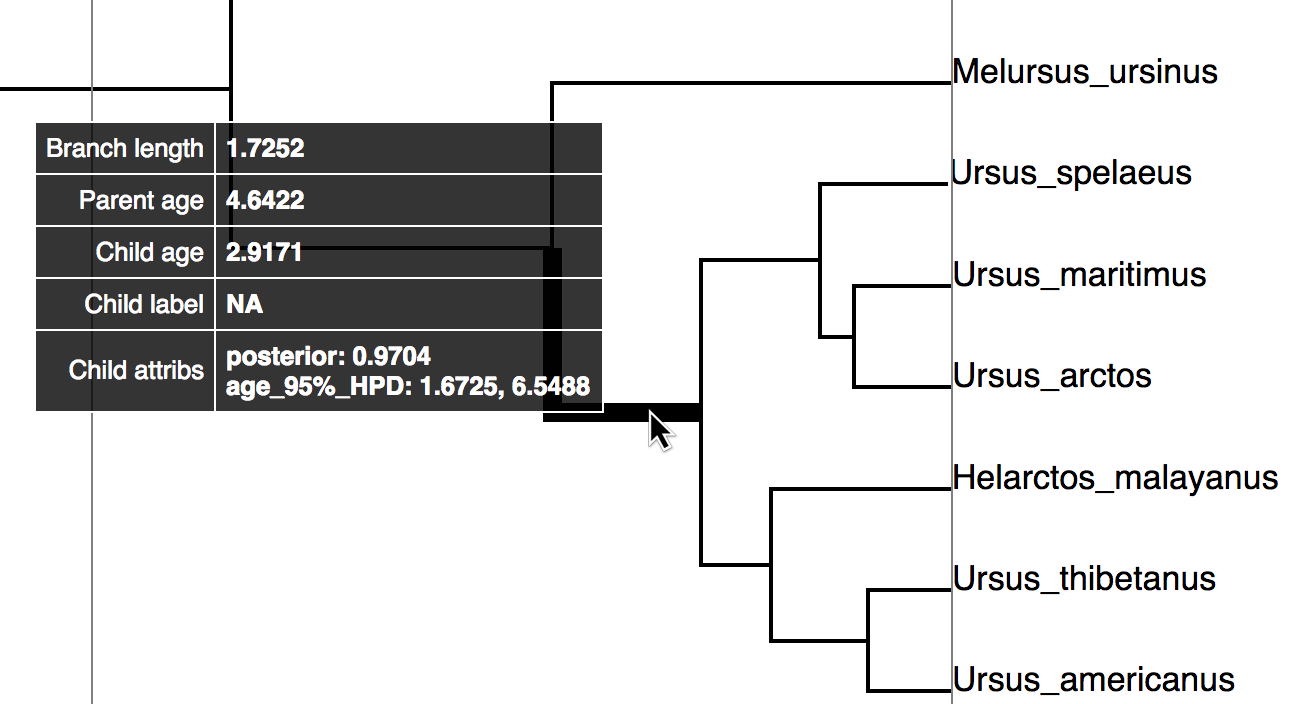
\includegraphics[scale=0.45, angle=0]{\ResourcePath figures/branch_highlight.png}
%\caption{\small Screenshot of highlighting a branch in {\tt IcyTree} showing child node attributes, including the clade posterior probability and the 95\% highest posterior density (HPD) age interval.}
%\end{minipage}}
%\label{fig:IcyTreeScreenshort}
%\end{figure}



%TODO IcyTree

\bibliographystyle{sysbio}
\bibliography{\GlobalResourcePath refs}
